\documentclass[aspectratio=169]{beamer}
\setbeamertemplate{navigation symbols}{}
\usepackage{color,amsmath,comment, subfigure}
\usepackage{booktabs}
\usepackage{url}

\def\imagetop#1{\vtop{\null\hbox{#1}}} %http://tex.stackexchange.com/questions/23521/tabular-vertical-alignment-to-top

%\setbeameroption{show notes}

%%%%%%%%%%%%%%%%%%%%%%%%%%
\title[]{Lecture 24: Online dating}
\author[]{Matthew J. Salganik}
\institute[]{Sociology 204: Social Networks\\Princeton University}
\date[]{1/2 Online dating

\vfill

\begin{flushleft}
\vspace{0.6in}

\includegraphics[width=0.1\textwidth]{figures/cc.png}
\end{flushleft}
}

\begin{document}
%%%%%%%%%%%%%%%%%%%%%%%%%%%
\frame{\titlepage}
%%%%%%%%%%%%%%%%%%%%%%%%%%%
\begin{frame}

Online dating create two kinds of question:
\begin{itemize}
\item How does online dating change dating and marriage?
\item How can we use online dating to study existing questions in new ways?
\end{itemize}

\vfill
This is a common pattern when new online systems are created.
 
\end{frame}
%%%%%%%%%%%%%%%%%%%%
\begin{frame}

How have sociologists studied dating and marriage in the past?
 
\end{frame}
%%%%%%%%%%%%%%%%%%%%
\begin{frame}

\begin{center}
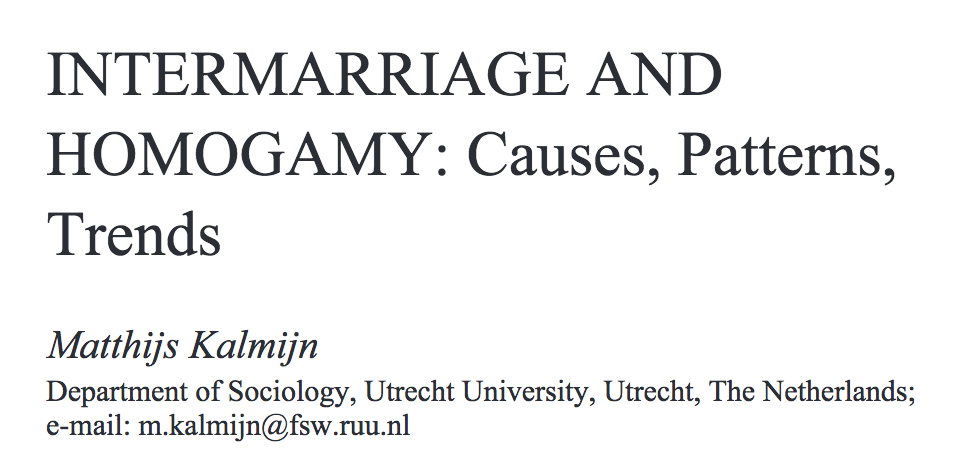
\includegraphics[width=0.5\textwidth]{figures/kalmijn_intermarriage_1998_title}
\end{center}

``People have a tendency to marry within their social group or to marry of person who is close to them in status.''  \pause
\begin{itemize}
\item Can we measure these patterns and see how it varies over time and across space?
\pause
\item Why does these pattern exist? (Very hard with only outcome data)
\end{itemize}

\vfill
\url{http://dx.doi.org/10.1146/annurev.soc.24.1.395}
\end{frame}
%%%%%%%%%%%%%%%%%%%%%%%%%%%
\begin{frame}

\begin{center}
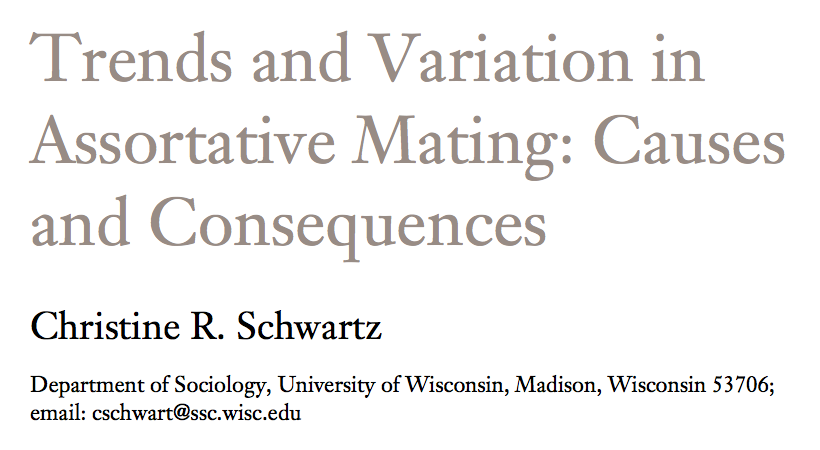
\includegraphics[width=0.5\textwidth]{figures/schwartz_trends_2013_title}
\end{center}

Consequences of assortative mating for:
\begin{itemize}
\item inequality within generations \pause
\item inequality between generations \pause
\item long-run population change \pause
\item relationship quality and dissolution
\end{itemize}

\vfill
\url{http://dx.doi.org/10.1146/annurev-soc-071312-145544}

\end{frame}
%%%%%%%%%%%%%%%%%%%%%%%%%%%
\begin{frame}

Now move to more process data, online and offline
\pause

\begin{center}
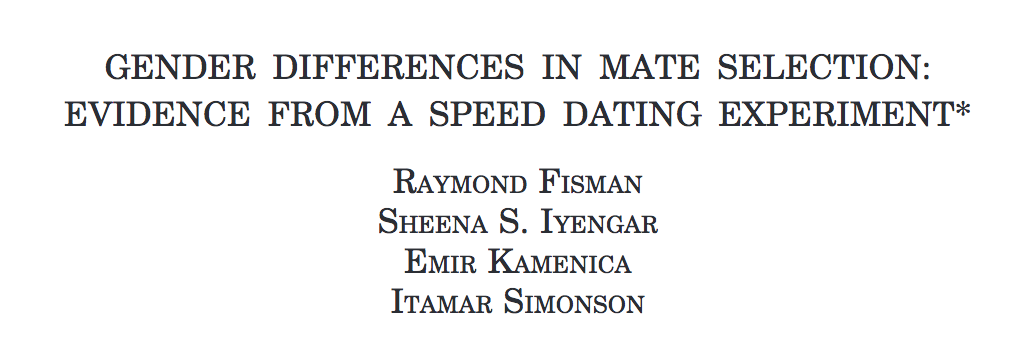
\includegraphics[width=0.95\textwidth]{figures/fisman_gender_2006_title}
\end{center}

\vfill

Observe all decisions, not just final matches

\note{
This is a speed dating study that I was in during grad school.  The researchers rented a room at a bar and we did speed dating.  Because of the context researchers asked us about our rating and decisions a lot.  This gave them process data not just outcome data.
}

\end{frame}
%%%%%%%%%%%%%%%%%%%%%%%%%%%
\begin{frame}

\begin{center}
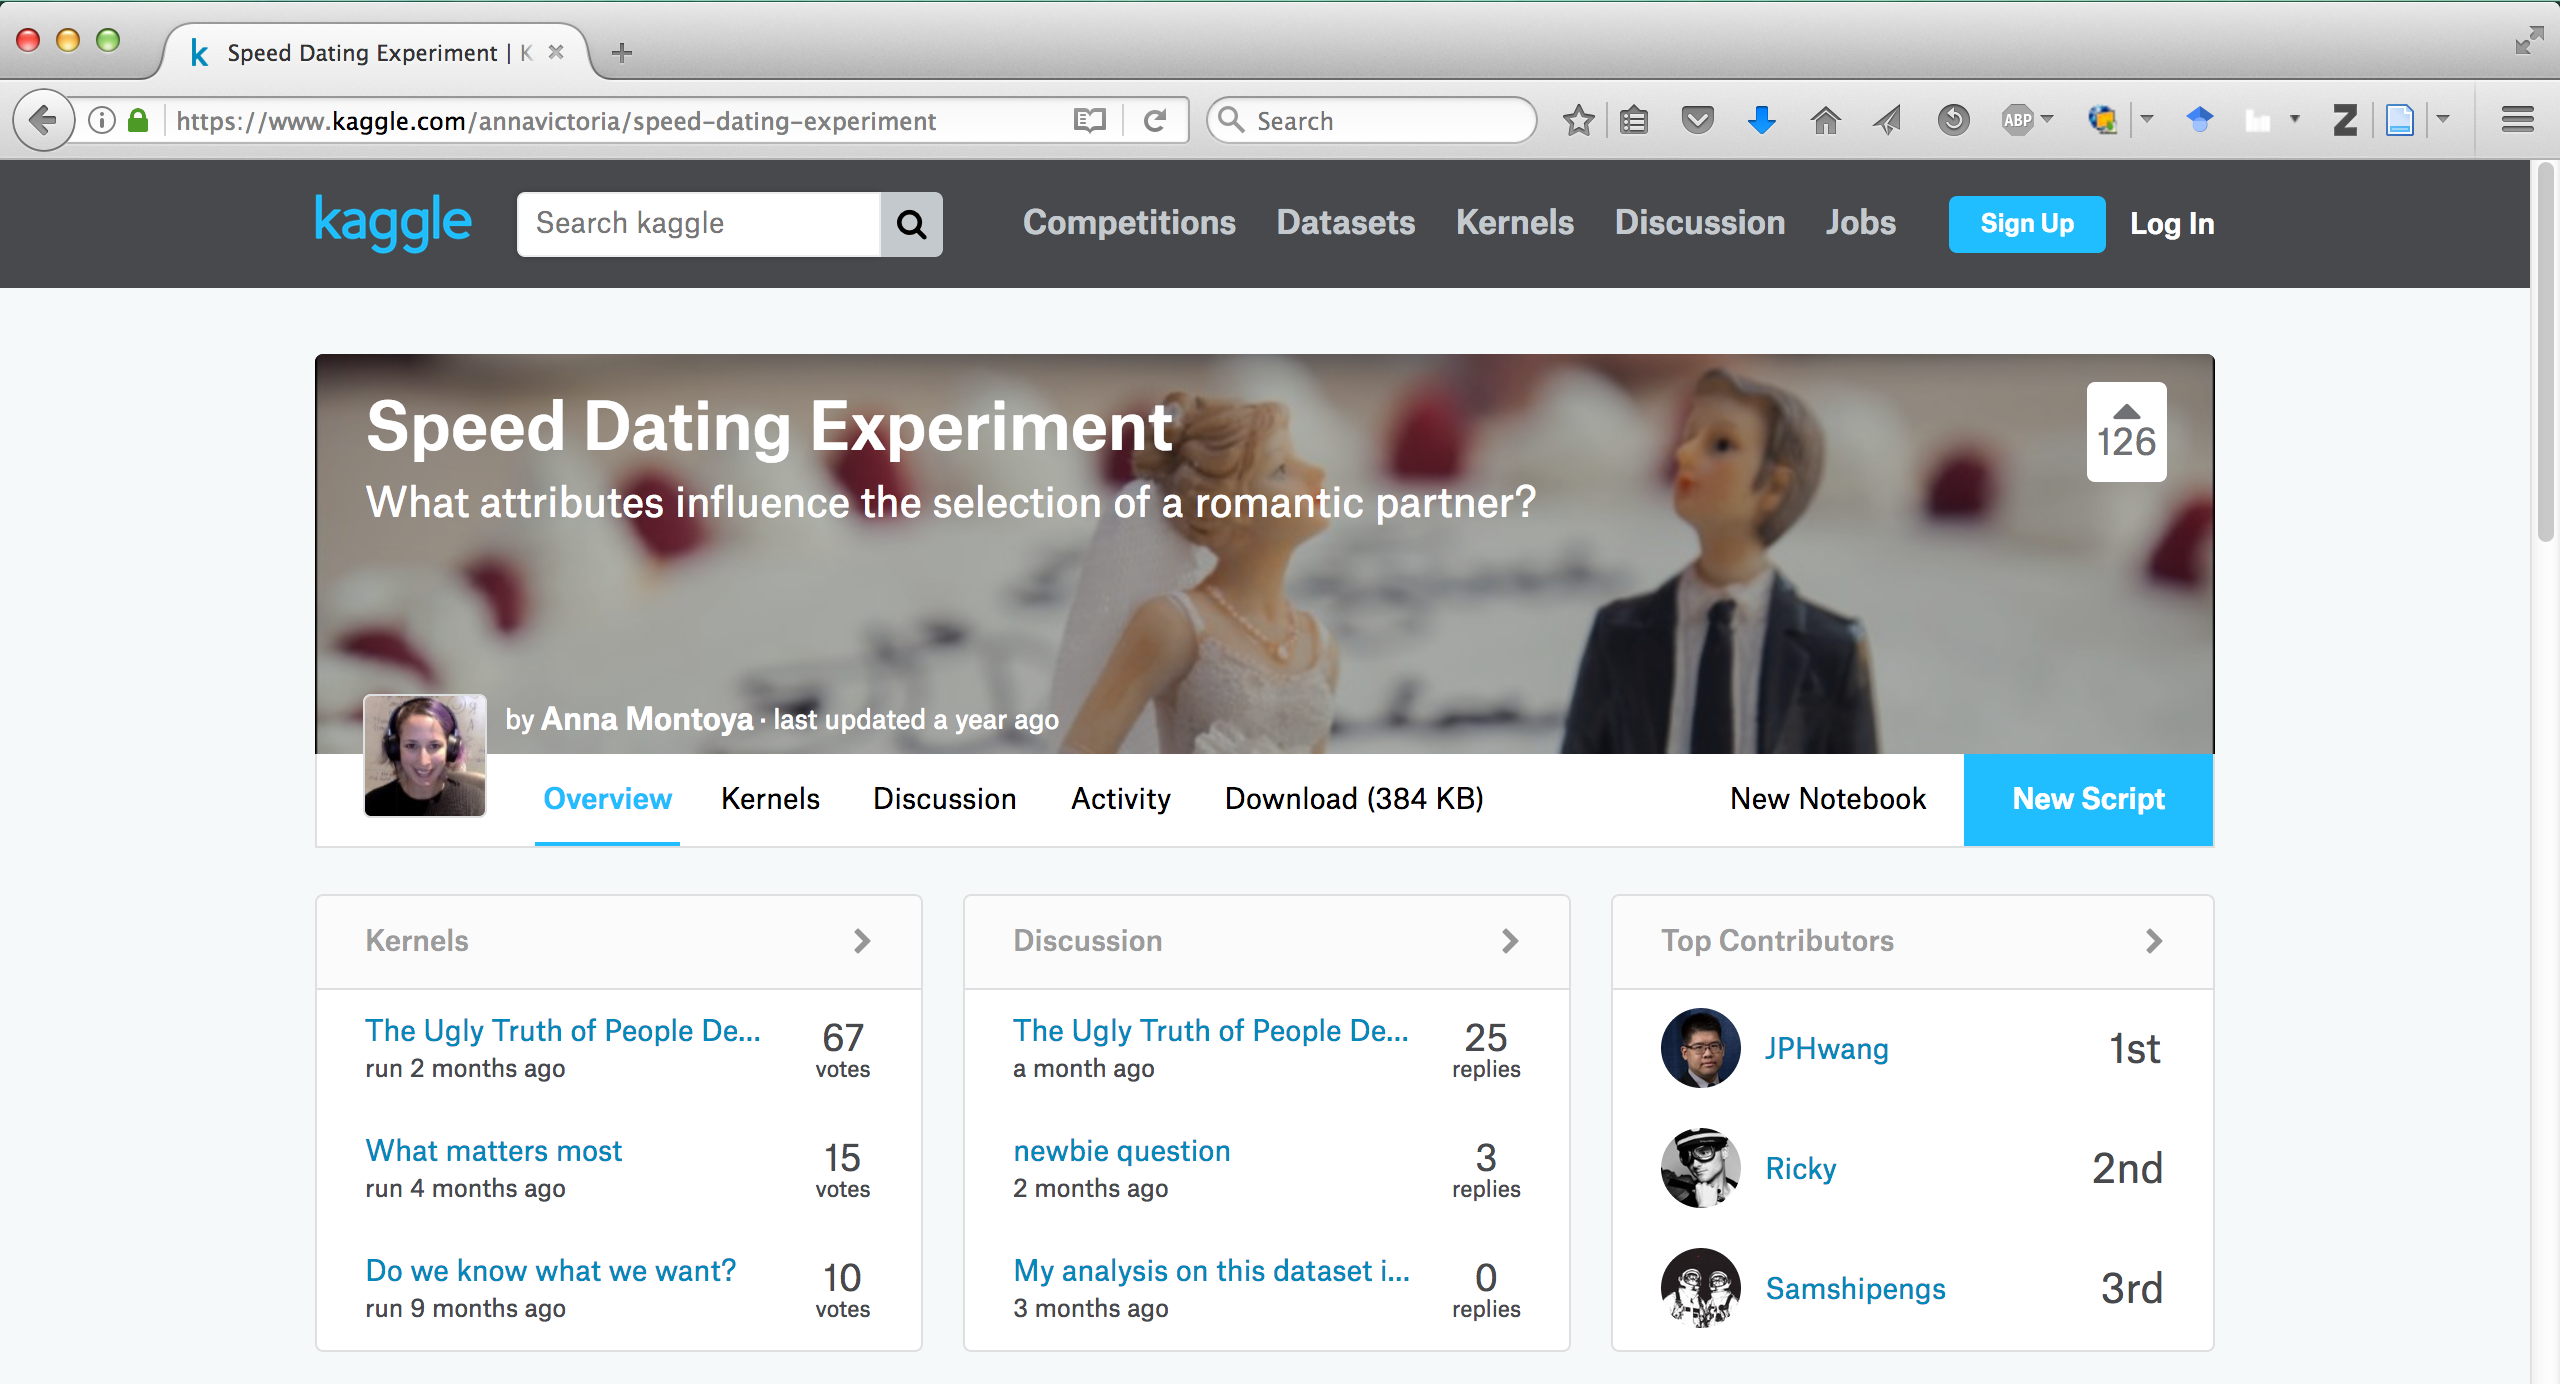
\includegraphics[width=0.95\textwidth]{figures/kaggle_speed_dating}
\end{center}

\url{https://www.kaggle.com/annavictoria/speed-dating-experiment}
\end{frame}
%%%%%%%%%%%%%%%%%%%%%%%%%%%
\begin{frame}

Online dating create two kinds of question:
\begin{itemize}
\item \textcolor{blue}{How does online dating change dating and marriage?}
\item How can we use online dating to study existing questions in new ways?
\end{itemize}

\end{frame}
%%%%%%%%%%%%%%%%%%%%
\begin{frame}

1940 heterosexual couples, US, way of meeting (some categories overlapped):
\begin{itemize}
\item family: 24 percent 
\item friends: 21 percent
\item school: 21 percent 
\item neighbors: 13 percent 
\item church: 13 percent
\item bar or restaurant: 12 percent 
\item co-workers: 10 percent 
\end{itemize}

\pause

By 2009, 
\begin{itemize}
\item half of all straight couples still met through friends or at a bar or restaurant, but 22 percent met online, and all other sources had shrunk. \pause
\item more than one-third of couples who married in the United States from 2005 to 2012 met online \pause
\item almost 70 percent of gay and lesbian couples met online
\end{itemize}

\vfill
\tiny{\url{https://www.nytimes.com/2015/06/14/opinion/sunday/how-to-make-online-dating-work.html}}

\end{frame}
%%%%%%%%%%%%%%%%%%%%%%%%%%%
\begin{frame}

\begin{center}
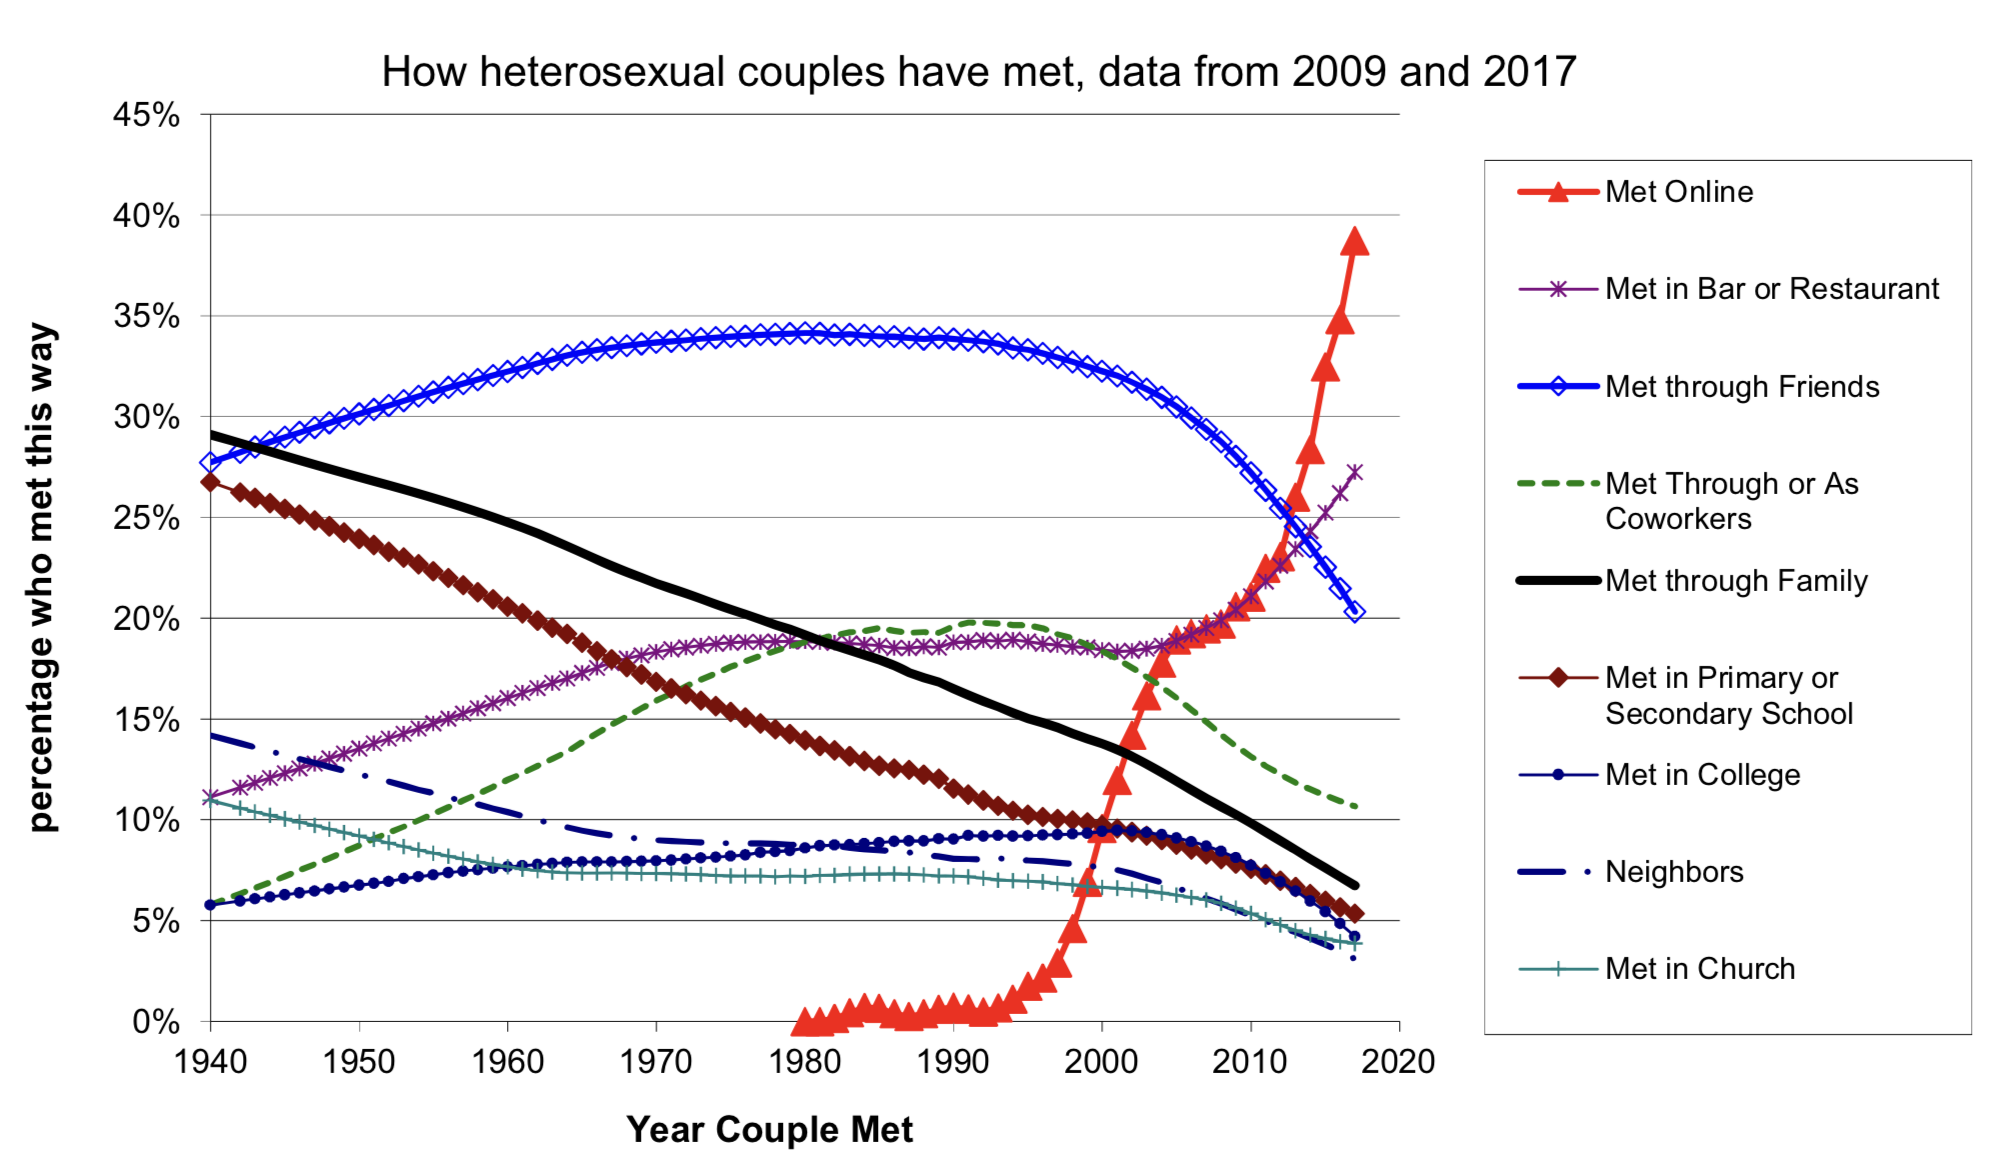
\includegraphics[width=0.95\textwidth]{figures/rosenfeld_disintermediating_2019_fig1}
\end{center}

\vfill
Source: Rosenfeld et al (2019) \url{https://doi.org/10.1073/pnas.1908630116}

\end{frame}
%%%%%%%%%%%%%%%%%%%%%%%%%
\begin{frame}

Online dating create two kinds of question:
\begin{itemize}
\item How does online dating change dating and marriage?
\item \textcolor{blue}{How can we use online dating to study existing questions in new ways?}
\end{itemize}

\end{frame}
%%%%%%%%%%%%%%%%%%%%
\begin{frame}

\begin{center}
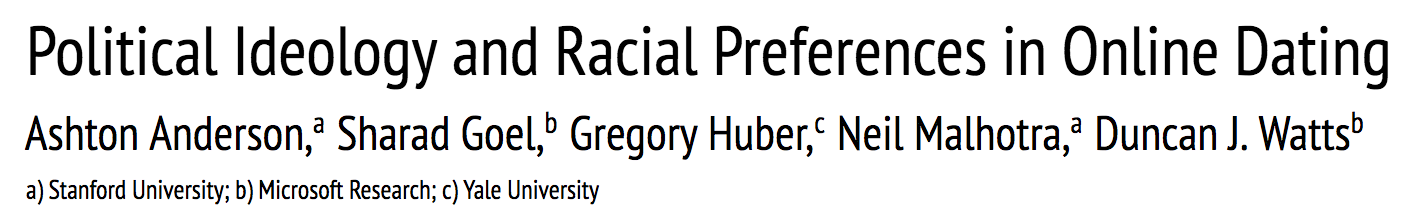
\includegraphics[width=0.9\textwidth]{figures/anderson_political_2014_title}
\end{center}

\vfill
\begin{itemize}
\item Focused on same race romantic relationships (racial homogamy). What are the roles of opportunity and choice?
\end{itemize}

\end{frame}
%%%%%%%%%%%%%%%%%%%%%%%%%%%
\begin{frame}

\begin{center}
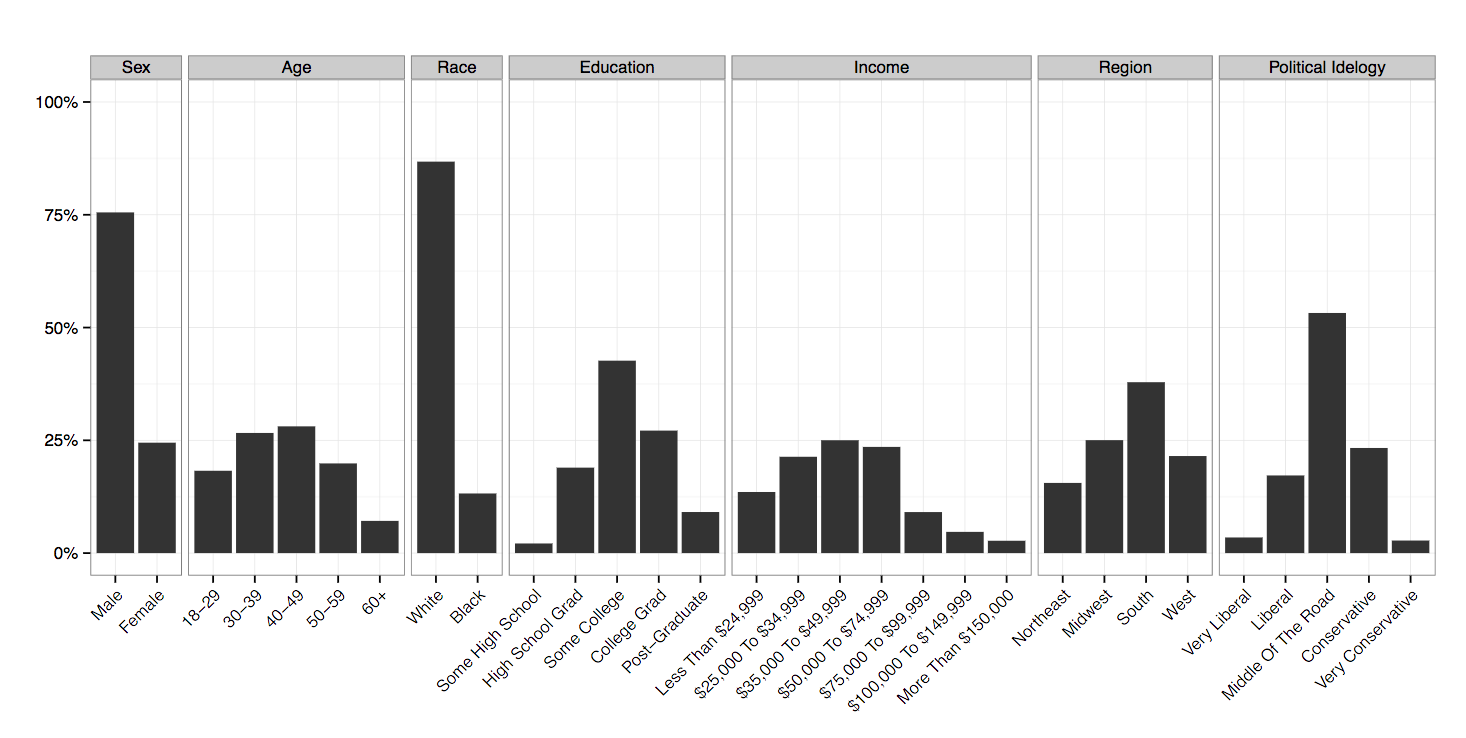
\includegraphics[width=0.8\textwidth]{figures/anderson_political_2014_fig1}
\end{center}

\pause
\vfill
\begin{itemize}
\item Analysis sample is limited to white and black heterosexuals. \pause Other research focuses on other groups. \pause
\item Sample is diverse in other ways.
\end{itemize}

\end{frame}
%%%%%%%%%%%%%%%%%%%%%%%%%%%
\begin{frame}

\begin{itemize}
\item Stated preferences: what you say you want
\item Revealed preferences: what you do
\end{itemize}

\end{frame}
%%%%%%%%%%%%%%%%%%%%%%%%%%%
\begin{frame}

\begin{center}
stated preferences
\end{center}

\end{frame}
%%%%%%%%%%%%%%%%%%%%%%%%%%%
\begin{frame}

\begin{center}
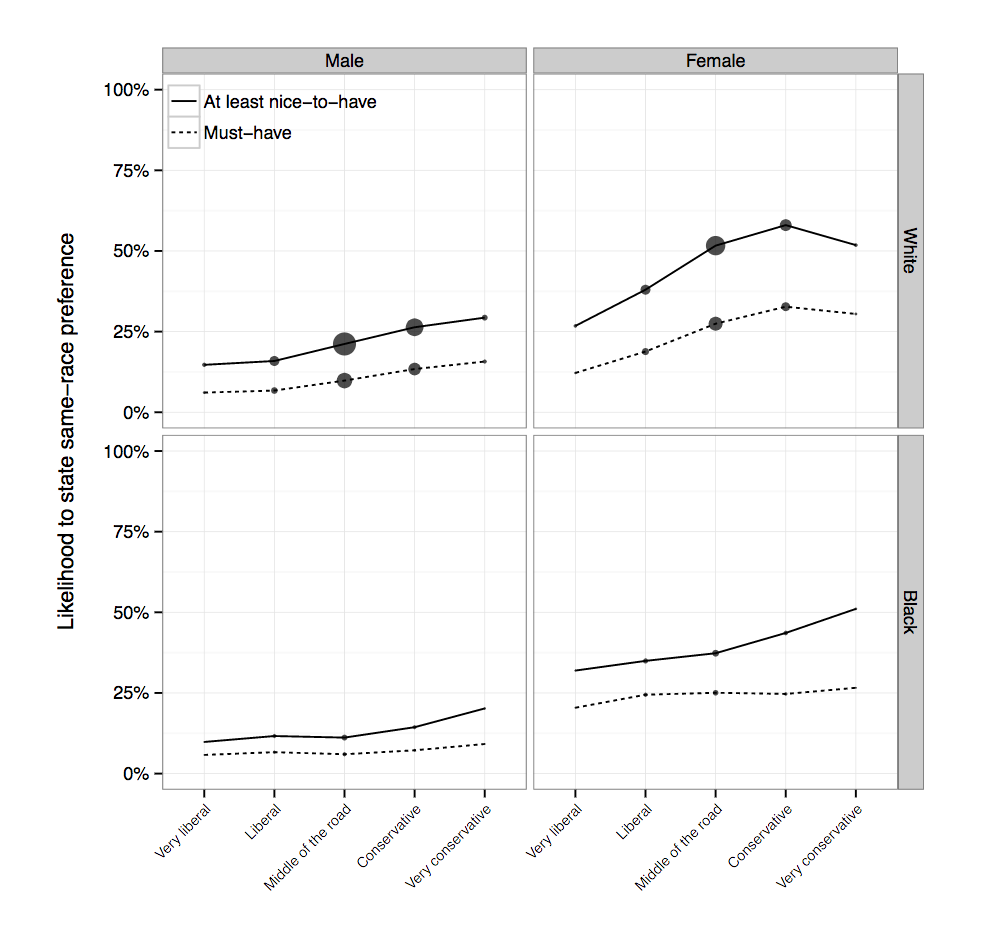
\includegraphics[width=0.5\textwidth]{figures/anderson_political_2014_fig2_top}
\end{center}

\pause
\begin{itemize}
\item Conservative show more stated preference for same-race partners \pause
\item Maybe this is caused by something correlated with conservativeness?  So, researchers do statistical adjustments.
\end{itemize}

\end{frame}
%%%%%%%%%%%%%%%%%%%%%%%%%%%
\begin{frame}

\begin{center}
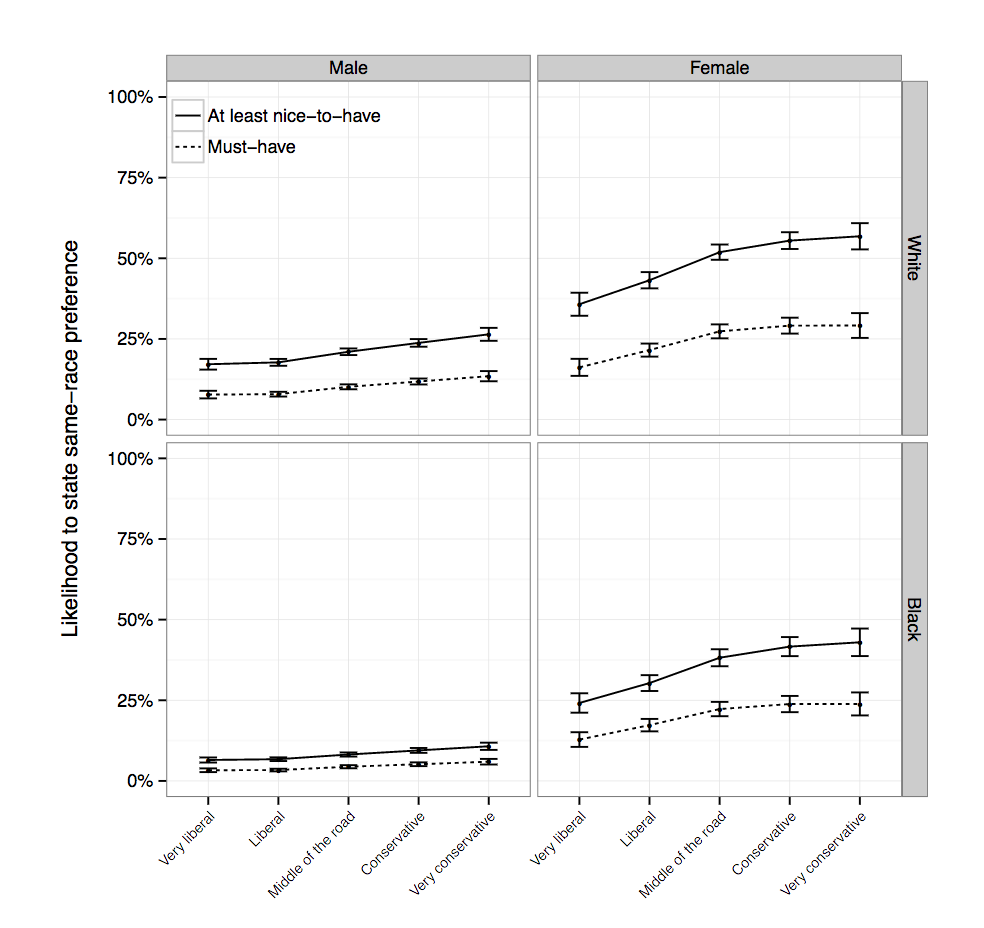
\includegraphics[width=0.5\textwidth]{figures/anderson_political_2014_fig2_bottom}
\end{center}

\pause
\begin{itemize}
\item Conservative show more stated preference for same-race partners, even after some statistical adjustments.
\end{itemize}

\end{frame}
%%%%%%%%%%%%%%%%%%%%%%%%%%%
\begin{frame}

\begin{center}
Revealed preferences
\end{center}

\end{frame}
%%%%%%%%%%%%%%%%%%%%%%%%%%%
\begin{frame}

\begin{center}
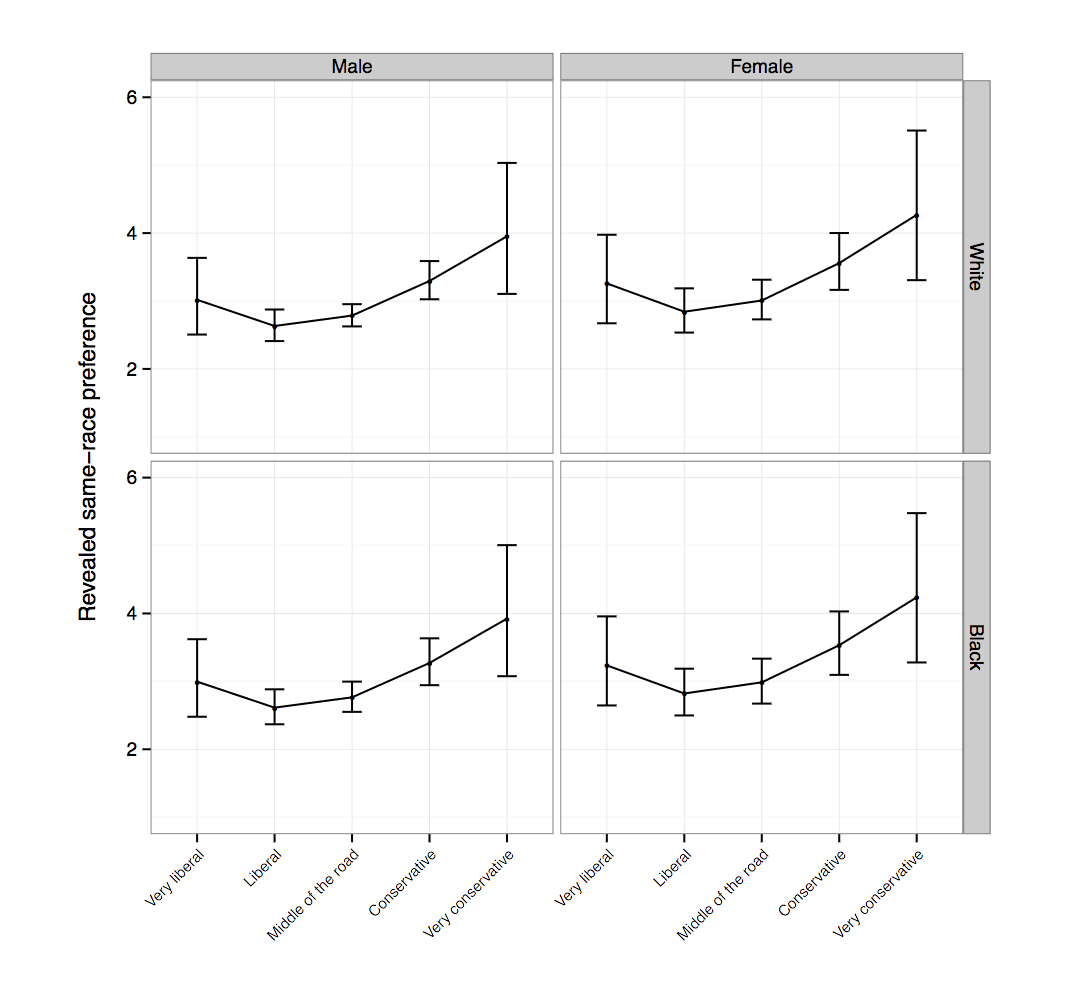
\includegraphics[width=0.4\textwidth]{figures/anderson_political_2014_fig4}
\end{center}
\vspace{-0.1in}
{\tiny
$\text{risk ratio} = \frac{Pr[q_i \text{ views profile of } c_i \mid q_i \text{ is the same race as } c_i ]}{Pr[q_i \text{ views profile of } c_i \mid q_i \text{ is different race as } c_i ]}$}

\pause
\begin{itemize}
\item More conservative individuals revealed preference to select same race partner \pause
\item Men and women are equally likely to have revealed preference to select same race partner
\end{itemize}
\end{frame}
%%%%%%%%%%%%%%%%%%%%%%%%%%%
\begin{frame}

\begin{center}
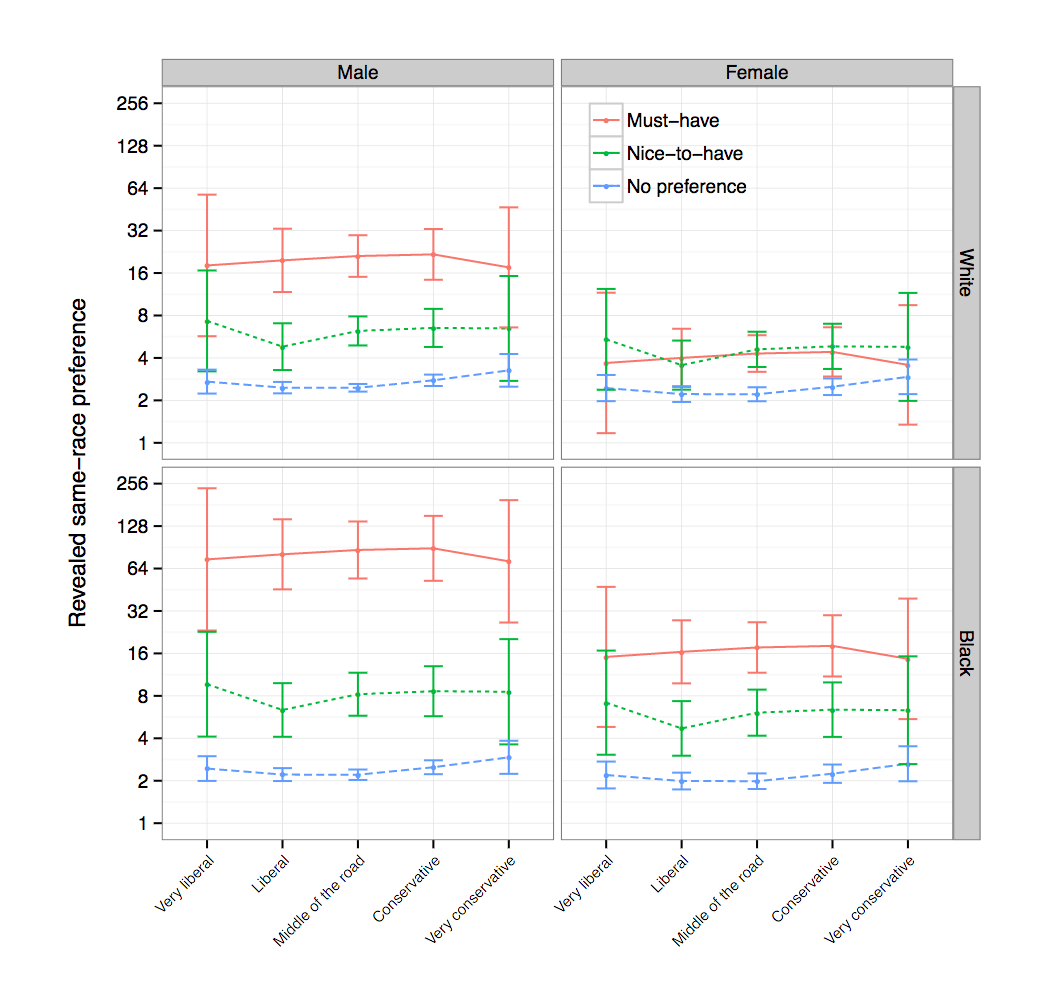
\includegraphics[width=0.4\textwidth]{figures/anderson_political_2014_fig5}
\end{center}
\vfill
\pause
\begin{itemize}
\item All groups exhibit revealed same-race preferences (note all estimates are above 1) \pause
\item People who have higher stated preferences have higher revealed preferences \pause
\item Not big differences by ideology
\end{itemize}

\end{frame}
%%%%%%%%%%%%%%%%%%%%%%%%%%%
\begin{frame}

\begin{center}
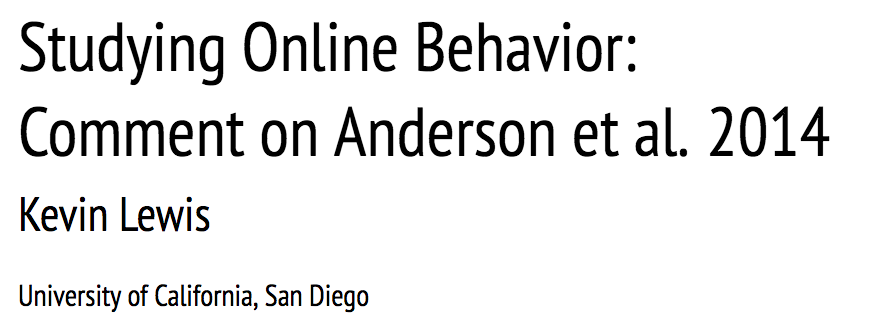
\includegraphics[width=0.7\textwidth]{figures/lewis_studying_2015_title}
\end{center}

\end{frame}
%%%%%%%%%%%%%%%%%%%%%%%%%%%
\begin{frame}

\begin{itemize}
\item Who is in their sample? Who isn't in their sample?
\pause
\item What kind of dating site? 
\pause
\item How much of these revealed preferences are the users and how much are the site's algorithms? (This should remind you of algorithmic filter bubbles).
\pause
\item Should we care about profile clicks or some other behavior, such as online contact or offline dating?
\end{itemize}

\end{frame}
%%%%%%%%%%%%%%%%%%%%%%%%%%%%
\begin{frame}

\begin{center}
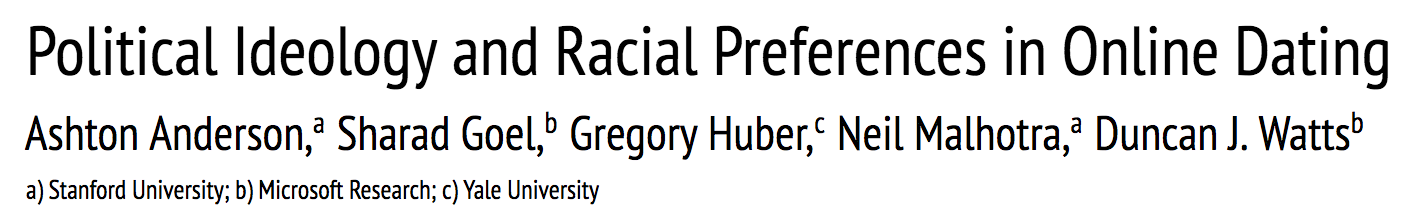
\includegraphics[height=0.2\textheight]{figures/anderson_political_2014_title}
\end{center}

\begin{center}
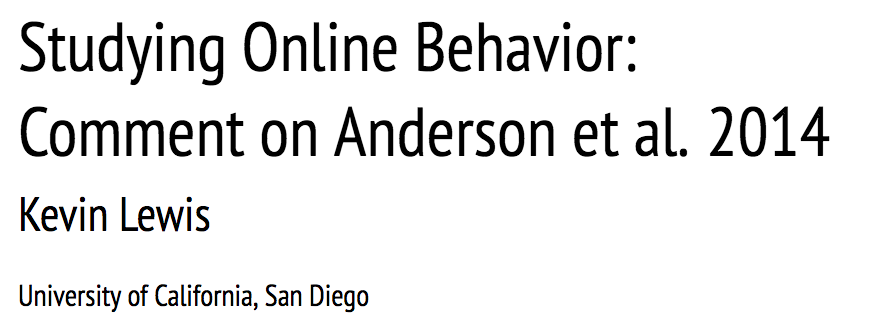
\includegraphics[height=0.3\textheight]{figures/lewis_studying_2015_title}
\end{center}

\begin{center}
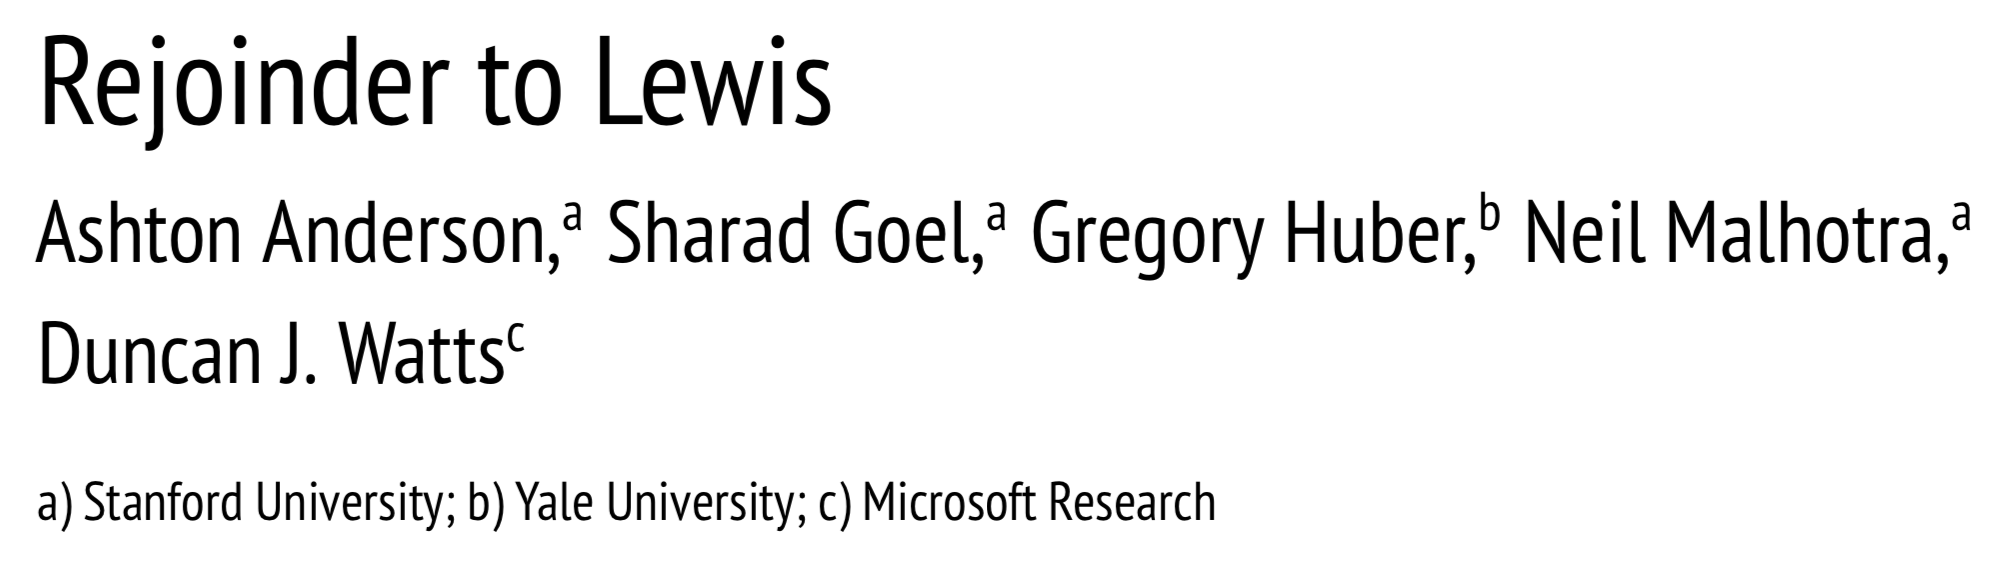
\includegraphics[height=0.3\textheight]{figures/anderson_rejoinder_2015_title}
\end{center}


\note{
How do we think about the three of these together.  Who is right and wrong?  I think they all make good points and these kind of debates help advance science.  If you found yourself thinking differently after reading each one that is progress.
}
 
\end{frame}
%%%%%%%%%%%%%%%%%%%%%%%%%%%%
\begin{frame}

Stepping back:
\begin{itemize}
\item racial homogomy is partially the results of opportunity and partially the result of choices \pause
\item online dating allows us to study those choices in more detail (but this can be tricky because of things like algorithmic confounding) \pause
\item in this study, participants had both stated and revealed preferences for same-race partners
\end{itemize}

\end{frame}
%%%%%%%%%%%%%%%%%%%%%%%%%%%%
\begin{frame}

Here are some more things to read about online dating:
\begin{itemize}
\item Lewis (2013) ``The limits of racial prejudice.'' \textit{PNAS}. \url{http://dx.doi.org/10.1073/pnas.1308501110}
\item Bruch et al (2016) ``Extracting multistage screening rules from online dating activity data.'' \textit{PNAS}. \url{http://dx.doi.org/10.1073/pnas.1522494113}
\item Huber and Malhotra (2017) ``Political Homophily in Social Relationships: Evidence from Online Dating Behavior.'' \textit{The Journal of Politics}, \url{http://dx.doi.org/10.1086/687533}.
\item Rafalow, Feliciano, and Robnett. 2017. ``Racialized Femininity and Masculinity in the Preferences of Online Same-Sex Daters.'' \textit{Social Currents}, \url{https://doi.org/10.1177/2329496516686621}
\item Rudder (2015) Datacylsm. \url{http://dataclysm.org/}
\item OKCupid Blog. \url{https://theblog.okcupid.com/}
\item Ansari and Klinenberg (2015) Modern Romance. \url{https://en.wikipedia.org/wiki/Modern_Romance:_An_Investigation}
\item Feliciano and Kizer (2020) ``Reinforcing the Racial Structure: Observed Race and Multiracial Internet Daters' Racial Preferences.'' \textit{Social Forces}, \url{https://doi.org/10.1093/sf/soaa065}
\end{itemize}

\end{frame}
%%%%%%%%%%%%%%

\end{document}
